% vim: set tw=78 sts=2 sw=2 ts=8 aw et ai:
\documentclass{workshop}

% Comentează liniile de mai jos în cazul în care nu există cod de inclus.
\usepackage{code/highlight}
\usepackage{color}        % dacă e folosit highlight
\usepackage{alltt}        % dacă e folosit highlight

\title[Sesssion 9]{Session 9}
\subtitle{Linux in Embedded Systems}
\author{Andrei Voinescu}
\date{12th July, 2012}

\begin{document}

% Arătăm numărul frame-ului
\setbeamertemplate{footline}[frame number]

\frame{\titlepage}

% NB: Secțiunile nu sunt marcate vizual, ci doar apar în cuprins
\section{Introduction}

\subsection{}

\begin{frame}{Introduction}
What we will be covering today
\begin{itemize}
	\item Why we use Linux in Embedded Systems
	\item How a Linux-capable board looks like
	\item How a Linux system boots up	
\end{itemize}
\visible<2->{What we will NOT be covering
\begin{itemize}
	\item How to develop Linux applications
	
\end{itemize}
}
\visible<3->{What we will experiment
\begin{itemize}
\item How to write a simple device driver for an embedded board
\item How to debug a module remotely via ssh
\end{itemize}
}
\end{frame}

\begin{frame}{Linux in the Embedded World}
\begin{itemize}
\item Linux exists in many embedded devices
	\begin{itemize}
		\item Routers, NASs, Displays
		\item Smartphones, tablets, ebook-readers
	\end{itemize}

\visible<2->{
\item .. But Why?
	\visible<3->{
	\begin{itemize}
		\item Linux kernel offers drivers for many commonly used components
		\item Complete networking stacks
		\visible<4->{
		\item Linux system offers many utilities and libraries
			\begin{itemize}
				\item coreutils
				\item SSH, http servers, mysql,...
			\end{itemize}

		\visible<5->{
		\item Many hypervisors already support Linux as a guest system
		}
		}
	\end{itemize}
}
}
\end{itemize}
\end{frame}

\section{Example of a Linux System}
\begin{frame}{ATNGW100}
\begin{figure}
	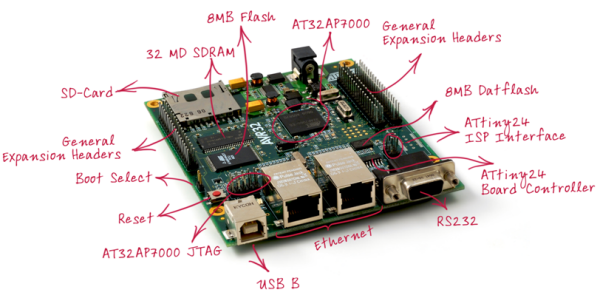
\includegraphics[width=1\textwidth]{img/Ngwoverview.png}
\end{figure}
\end{frame}

\section{Booting Up}

\section{Practical}

\end{document}
